\documentclass[a4paper, 11pt]{article}
\usepackage[T1]{fontenc}
\usepackage[utf8]{inputenc}
\usepackage[french]{babel}
\usepackage{verbatim}
\usepackage{graphicx}
\begin{document}

\title{Projet d'Algorithmique}
\author{David Galichet et Baptiste Fontaine}
\date{29 novembre 2013}
\maketitle
\newpage
\tableofcontents
\newpage


\part{Implémentation}

Le projet a été écrit avec Python 3 sans utilisation de bibliothèques externes.
Il est versionné avec Git et sera disponible en ligne à la fin du semestre.

\section{Mise en route}
\subsection{Installation}

Le code est situé dans \verb|src|, et ne nécessite pas d'installation
particulière. Assurez-vous cependant d'avoir au moins Python 3.1.

Un \verb|Makefile| est fourni afin de compiler le présent rapport
(\verb|make report|) et de faire tourner la suite de tests (\verb|make check|).
Sous réserve d'avoir installé le module \verb|coverage| pour Python 3,
\verb|make checkcover| permet de vérifier la couverture du code par ces tests,
qui est d'au moins 90\%.  La suite de test vérifie que les fonctions de gestion
des algorithmes fonctionnent bien, et fait passer une série de tests à chaque
algorithme qui vérifie que chacun ne donne que des solutions valides (i.e.
préserve tous les mots dans l'ordre et ne génère pas de lignes trop longues).

\subsection{Utilisation}

Le programme s'appelle \verb|wrapper|, il suffit de le lancer avec l'option
\verb|--help| pour avoir un aperçu de son utilisation ainsi qu'une liste des
algorithmes disponibles. Il lit son entrée sur l'entrée standard, et écrit le
résultat sur la sortie standard. Il est possible de choisir l'algorithme à
utiliser en utilisant l'option \verb|--algo|, ainsi que de changer la largeur
de la page (79 par défaut) avec \verb|-w|. Le texte en sortie peut être
justifié avec l'option \verb|--justify|.

Par exemple, pour utiliser l'algorithme \ref{sec:simple-greedy} avec une largeur
de page de 76 pour un texte situé dans \verb|in.txt|, utilisez la ligne suivante
:

\begin{verbatim}
./wrapper --algo greedy -w 76 < in.txt
\end{verbatim}

Il est également possible d'obtenir plus d'informations sur un algorithme en
utilisant l'option \verb|--info|.

\begin{verbatim}
./wrapper --info greedy
\end{verbatim}

\section{Fonctionnement}

Un des avantages de Python par rapport aux autres langages proposés pour ce
projet est qu'il a des fonctions de première classe. Nous avons utilisé cette
fonctionalité ainsi que le chargement dynamique de modules pour avoir un
environnement permettant de très facilement ajouter ou enlever des algorithmes
sans avoir à modifier aucune autre partie du code que la fonction qui définit
l'algorithme.

Lors du lancement du programme, tous les modules Python situés dans
\verb|src/algos| sont chargés et les fonctions implémentant des algorithmes
qu'ils contiennent sont enregistrées dans une table de correspondance, qui
associe leur nom avec leur fonction et la documentation optionnelle. En fonction
des options données sur la ligne de commande, le programme utilise ensuite cette
table pour afficher la liste des algorithmes possibles, afficher la
documentation de l'un d'eux ou l'exécuter sur du texte donné en entrée.

Chaque algorithme est défini sous forme d'une fonction qui prend en argument une
liste paresseuse de mots (un générateur) et une largeur, et génère une liste
de lignes qui correspond au texte imprimé sur une page de la largeur donnée.
Nous utilisons les décorateurs de Python pour différencier les fonctions qui
implémentent des algorithmes des fonctions auxilliaires. Chaque ligne est
retournée comme une liste de mots, de façon à simplifier l'éventuelle
justification.

Voici par exemple ce que serait le code déclarant un algorithme qui affiche un
mot par ligne, peut importe la largeur de la page :

\begin{verbatim}
@algo("An example algorithm")
def one_word_per_line(words, width):
    """
    This algorithm is an example,
    don't use it! It outputs only one word
    per line.
    """
    for word in words:
        yield [word] # one line
\end{verbatim}

Cet algorithme pourrait ensuite être utilisé sur la ligne de commande :

\begin{verbatim}
$ ./wrapper --info one-word-per-line
One Word Per Line: An example algorithm

    This algorithm is an example,
    don't use it! It outputs only one word
    per line.

$ echo foo bar | ./wrapper -a one-word-per-line -w 42
foo
bar
\end{verbatim}

\part{Algorithmes}

Les algorithmes sont regroupés par familles, telles que vues en cours.
La complexité théorique dans le pire des cas est donnée en fonction de la
longueur du texte en entrée ($n$) et de la largeur maximale d'une ligne ($k$).
Chaque algorithme a une complexité d'au moins $O(n)$ en temps car il faut dans
tous les cas calculer la longueur de chaque mot. En pratique, nos fonctions
génèrent des lignes à afficher, donc leur complexité en mémoire est toujours
d'au moins $O(k)$ car elles ont toujours au moins une ligne en mémoire. Nous
nous intéressons ici uniquement à la complexité théorique.

Dans le cas particulier où un mot serait plus long que la largeur de la page, le
programme affiche une erreur, ce qui permet de ne pas se préoccuper de ce cas
dans les implémentations d'algorithmes puisque le problème est géré en amont.

Nous avons ajouté une méthode de justification du texte (i.e. insertion
d'espaces entre les mots de façon à ce que chaque ligne prenne la place
maximale) qui s'applique en repassant sur le texte formatté. Cette méthode est
décrite dans la section \ref{sec:justification}.

\section{Diviser pour régner}

\subsection{Algorithme naïf}

Cet algorithme est une implémentation naïve du principe de « diviser pour régner
», en effet il ne fait que diviser par deux récursivement le texte donné en
entrée jusqu'à ce que chaque partie puisse tenir sur une ligne. Il ne fonctionne
donc que sur des textes de longueur raisonnable puisque sa complexité en mémoire
est en $O(n)$ car tout le texte doit être lu avant de pouvoir le diviser.
L'utilité du « diviser pour régner » est discutable ici, puisque tous les mots
doivent être lus car il faut connaître leur longueur. La complexité n'est donc
pas réduite par l'utilisation de ce type d'algorithme. Elle est de
$O(n+\log_2 n) \in O(n)$ (parcours de l'ensemble du texte en entrée et division
du tableau). La lisibilité du texte généré est plus faible qu'avec les autres
algorithmes, car il y a beaucoup d'espaces de fin de ligne.

Utilisez \verb|naive-dc| pour tester l'algorithme.

\subsection{Algorithme alternatif}

Cet algorithme fonctionne de façon similaire au précédent, mais dans certains
cas génère un résultat différent. Il divise récursivement la liste de mot en
entrée en deux jusqu'à n'avoir que des listes composées d'un seul mot chacune.
Ensuite, il « remonte » jusqu'à la solution en concaténant les listes de mots
jusqu'à ce qu'une concaténation soit la plus longue possible pour une ligne
(i.e. concaténer cette liste avec une autre dépasserait de la ligne). Il a les
mêmes complexités en temps et mémoire que le précédent algorithme, mais donne un
texte plus lisible, bien que restant inférieur aux algorithmes dynamiques
présentés en section \ref{sec:dynprog}.

Utilisez \verb|alternative-dc| pour tester l'algorithme.

\section{Gloutons}

\subsection{Algorithme simple}
\label{sec:simple-greedy}

Cet algorithme, qui marche en $O(n)$ ($O(1)$ pour la mémoire), est le plus
intuitif et le plus simple à implémenter. Il ajoute tous les mots à la suite
tant qu'il a assez de place sur une ligne, puis passe à la suivante.

Utilisez \verb|greedy| le tester.

\subsection{Algorithme balancé}
\label{sec:balanced-greedy}

Cet algorithme est une variante de l'algorithme glouton simple
(\ref{sec:simple-greedy}) qui ajoute des espaces entre les mots dans le but de
balancer le texte pour réduire la quantité d'espaces en fin de ligne. Il est
inspiré de la méthode de Samet \cite{Samet82} qui cherche à répartir les espaces
dans un paragraphe justifié. Ici, l'algorithme effectue une première passe en
utilisant \ref{sec:simple-greedy}, puis calcule la largeur moyenne des espaces
inter-mots du texte, comme s'il était justifié. Il repasse ensuite sur le texte
et ajoute des espaces aux mots de façon à ce que chaque espace inter-mot ai une
largeur proche de la moyenne. Il effectue enfin une seconde passe avec
l'algorithme glouton simple car des mots peuvent avoir été poussés vers la ligne
suivante à cause de l'ajout d'espaces.

Il est possible de tester cet algorithme avec \verb|balanced-greedy|. Il
marche en $O(3n)$ en temps, et $O(n)$ en mémoire. Le résultat est généralement
moins bon visuellement qu'avec \ref{sec:simple-greedy} car il y a plus d'espaces
et plus de lignes utilisées.

\section{Programmation dynamique}
\label{sec:dynprog}

\subsection{Algorithme de Knuth}

Nous avons implémenté deux variantes de l'algorithme de Knuth \cite{Knuth81}.
L'algorithme associe une pénalité à un texte en fonction du nombre d'espaces en
fin de ligne. La variante \verb|dynamic-2| utilise la somme des carrés des
espaces en fin de ligne, tandis que la variante \verb|dynamic-3| utilise la
somme des cubes. Le but est de minimiser la pénalité associée à un texte, et ce
en utilisant la programmation dynamique.

Le but est ici de remplir un tableau $T_1$ où chaque case $(i, j)$ représente le
coût d'une ligne contenant les mots $w_i$ à $w_j$ (avec $i,j\ge 0$ et $i\le j$).
Ce coût est nul si la ligne tient parfaitement dans la largeur de page donnée,
infini si la ligne est trop grande, et est fonction du nombre d'espaces restants
sinon. On construit ensuite un tableau $T_2$, où $T_2[i]$ contient le coût
optimal de l'arrangement des mots $w_0$ à $w_i$. Le coût optimal pour le texte
donné est ensuite situé en $T_2[n]$ (où $n$ est l'indice du dernier mot du
texte).

C'est l'algorithme qui donne les meilleurs résultats visuellement\footnote{les
deux variantes implémentées ne génèrent pas de solutions significativement
différentes. Nous les avons gardés pour montrer qu'il est possible de changer le
poids associé aux espaces en fin de ligne pour faire varier légèrement le texte
généré.}. Par contre, c'est également l'algorithme qui a la pire complexité
en mémoire, puisqu'elle est de $O(n^2)$ car le tableau $T_n$ est de taille $n
\times n$.

Il a une complexité en temps de $O(n^2)$. On pourrait la réduire à $O(kn)$
en prenant en compte le fait que pour une largeur $k$ donnée, on ne peut
placer au maximum que $\lceil \frac{k}{2} \rceil$ mots dessus car ils sont
toujours séparés par un espaces, et dans le meilleur des cas ils ont tous une
largeur égale à 1.

\section{Backtracking}

Nous avons implémenté un algorithme qui utilise une logique similaire à
l'algorithme dynamique puisqu'il associe un coût à un paragraphe qui dépend du
nombre d'espaces en fin de ligne, mais qui cherche une solution optimale en
utilisant du backtracking. On obtient ici du texte lisible mais en beaucoup plus
de temps qu'avec les autres algorithmes. Il a une complexité en mémoire de
$O(3n)$ car il a besoin de tous les mots ainsi que de deux tableaux auxilliaires
le temps du calcul. Il a une complexité en temps de $O(\frac{n^3}{k})$, ce qui
fait qu'il est particulièrement inefficace sur des textes avec une faible
largeur.

Il peut être testé avec \verb|backtracking|.

\section{Justification}
\label{sec:justification}

Bien que le sujet ne la mentionne pas et que la justification de texte puisse
poser des problèmes \cite{Van96cognitive} notamment à cause de l'insertion de
nombreux espaces entre les mots\footnote{Ce qui peut créer des « rivières » ou
« lézardes », qui en typographie sont des suites verticales d'espaces entre les
mots qui forment des chemins blancs dans le texte et distraient l'œil
\cite{Harkins12fr}, comme les trous blancs.}, il nous a parut intéressant de
nous pencher sur ce problème. La justification se fait une fois tous les mots
disposés sur les lignes en ajustant les espaces inter-mots de façon à ce que le
texte soit aligné aussi bien à gauche qu'à droite.

L'algorithme fonctionne ligne par ligne. Il calcule le nombre d'espaces en trop
en fin de ligne et les répartie équitablement entre les mots de gauche à droite.

Cet algorithme est indépendant des autres, et peut être testé en ajoutant
l'option \verb|--justify| sur la ligne de commande, ce qui a pour effet de
justifier le texte produit par l'algorithme demandé.

Il ajoute une complexité en $O(2n)$ en temps (il passe une première fois sur une
ligne pour calculer le nombre d'espaces à sa fin, puis une seconde pour les
répartir, et ce pour chaque ligne), et $O(k)$ en mémoire puisqu'il ne garde
qu'une seule ligne en mémoire à chaque fois.

\part{Tests}

\section{Temps d'exécution}

Le tableau ci-dessous récapitule les complexités théoriques de chacun des
algorithmes, et inclut le résultat de mesures effectuées sur un texte avec deux
largeurs différentes. Le texte comporte 400 mots; le premier test utilise une
largeur de 15 tandis que le second utilise une largeur de 70. Les tests ont été
effectués sur un MacBook Air 2013, processeur 1,3 GHz Intel Core i5, en
exécutant chaque algorithme 100 fois pour chaque largeur, sur un texte de 400
mots. Les temps sont donnés en secondes.

On notera que certains résultats peuvent être faussés à cause du compilateur JIT
de Python qui optimise certaines parties du code. Ainsi, dans le tableau
ci-dessous, l'algorithme glouton balancé est plus rapide que l'algorithme
glouton alors qu'il a le triple de sa complexité en temps.

\begin{figure}[!h]
\begin{tabular}{|l|c|c|c|c|c|}
    \hline
    Algorithme & Temps & Mémoire & Lisibilité & Lorem15 & Lorem70 \\
    \hline
    diviser naïf & $O(n)$ & $O(n)$ & très basse & 5.36 & 5.40 \\
    diviser alternatif & $O(n)$ & $O(n)$ & basse & 5.24 & 5.41 \\
    glouton & $O(n)$ & $O(1)$ & moyenne & 5.47 & 5.40 \\
    glouton balancé & $O(3n)$ & $O(n)$ & basse & 5.28 & 5.35 \\
    dynamic-2 & $O(n^2)$ & $O(n^2)$ & très bonne & 5.30 & 12.06 \\
    dynamic-3 & $O(n^2)$ & $O(n^2)$ & très bonne & 5.77 & 12.51 \\
backtracking & $O(\frac{n^3}{k})$ & $O(3n)$ & bonne & $\infty$ & 84.35 \\
    justification & $O(2n)$ & $O(k)$ & - & - & - \\
    \hline
\end{tabular}
\caption{Comparaison des différents algorithmes}
\end{figure}

Comme on peut le voir dans ce tableau récapitulatif, il n'y a pas d'algorithme
qui donne une solution optimale sans être coûteux en temps et en mémoire. Sur de
courts textes, on pourra utiliser l'approche dynamique, mais sur de plus longs
textes l'algorithme glouton permettra d'avoir une relativement bonne lisibilité
en gardant une complexité linéaire en temps et constante en mémoire.

Nous avons dû interrompre le test de l'algorithme de backtracking sur un texte
de largeur 15 car il prenait bien trop de temps.

\section{Largeur de ligne}

Nous avons testé chaque algorithme sur un texte donné avec une largeur de ligne
entre 10 et 100, pour voir comment évoluaient les temps d'exécution. Sans
surprise, il n'y a que l'algorithme de backtracking qui voit son temps
d'exécution changer.

Le graphique ci-dessous montre le résultat d'un test avec cet algorithme.  Notre
script l'a exécuté sur un texte de 400 mots et une largeur décroissante jusqu'à
ce que l'exécution dure trop longtemps. Les valeurs en ordonnées sont des
nombres de secondes. On voit clairement la croissance exponentielle du temps
d'exécution quand la largeur approche les 15 caractères\footnote{La valeur
exacte importe peu, seul le comportement général nous intéresse ici}.

\begin{figure}[!h]
    \centering
    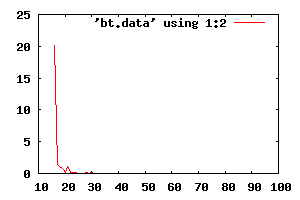
\includegraphics{bt.png}
    \caption{Backtracking en fonction de la largeur de ligne}
\end{figure}

\part{Résultats}

On trouvera ici un exemple de résultat pour chaque algorithme sur le même texte
en entrée et une largeur de 40. Voici le texte non formatté :

\begin{verbatim}
Il vaut mieux pomper même s’il ne se passe rien que de risquer
qu’il se passe quelque chose de pire en ne pompant pas, en tout
cas c'est ce que dit mon cousin Robert.
\end{verbatim}

Certains algorithmes ont un résultat identique avec ce texte et cette largeur,
mais peuvent différer avec d'autres conditions.

\begin{figure}[!h]
\begin{verbatim}
Il vaut mieux pomper même s’il ne se
passe rien que de
risquer qu’il se passe quelque
chose de pire en ne pompant pas, en
tout cas c'est ce
que dit mon cousin Robert.
\end{verbatim}
\caption{« Diviser pour régner » naïf}
\end{figure}

\begin{figure}[!h]
\begin{verbatim}
Il vaut mieux pomper même
s’il ne se passe
rien que de risquer
qu’il se passe quelque
chose de pire en ne pompant pas, en tout
cas c'est ce que dit mon cousin Robert.
\end{verbatim}
\caption{« Diviser pour régner » alternatif}
\end{figure}

\begin{figure}[!h]
\begin{verbatim}
Il vaut mieux pomper même s’il ne se
passe rien que de risquer qu’il se passe
quelque chose de pire en ne pompant pas,
en tout cas c'est ce que dit mon cousin
Robert.
\end{verbatim}
\caption{Glouton}
\end{figure}

\begin{figure}[!h]
\begin{verbatim}
Il  vaut  mieux  pomper  même  s’il  ne
se passe  rien  que  de  risquer  qu’il
se  passe quelque  chose  de  pire  en
ne  pompant  pas, en  tout  cas  c'est
ce  que  dit  mon  cousin Robert.
\end{verbatim}
\caption{Glouton balancé}
\end{figure}

\begin{figure}[!h]
\begin{verbatim}
Il vaut mieux pomper même s’il ne se
passe rien que de risquer qu’il se passe
quelque chose de pire en ne pompant pas,
en tout cas c'est ce que dit mon cousin
Robert.
\end{verbatim}
\caption{Programmation dynamique}
\end{figure}

\begin{figure}[!h]
\begin{verbatim}
Il vaut mieux pomper même s’il ne se
passe rien que de risquer qu’il se passe
quelque chose de pire en ne pompant pas,
en tout cas c'est ce que dit mon cousin
Robert.
\end{verbatim}
\caption{Backtracking}
\end{figure}

\begin{figure}[!h]
\begin{verbatim}
Il  vaut  mieux  pomper  même s’il ne se
passe rien que de risquer qu’il se passe
quelque chose de pire en ne pompant pas,
en  tout cas c'est ce que dit mon cousin
Robert.
\end{verbatim}
\caption{Glouton avec justification}
\end{figure}

\newpage
\bibliographystyle{plain}
\bibliography{rapport}
\end{document}
